%!TEX root = ../my_thesis.tex

\section[$\Bz\to\Dmp\pipm$ analysis motivation and phenomenology]{\boldmath{$\Bz\to\Dmp\pipm$} analysis motivation and phenomenology}
\label{sec:intro}
\setlength{\textfloatsep}{30pt}
\begin{figure}[t]
        \begin{center}
                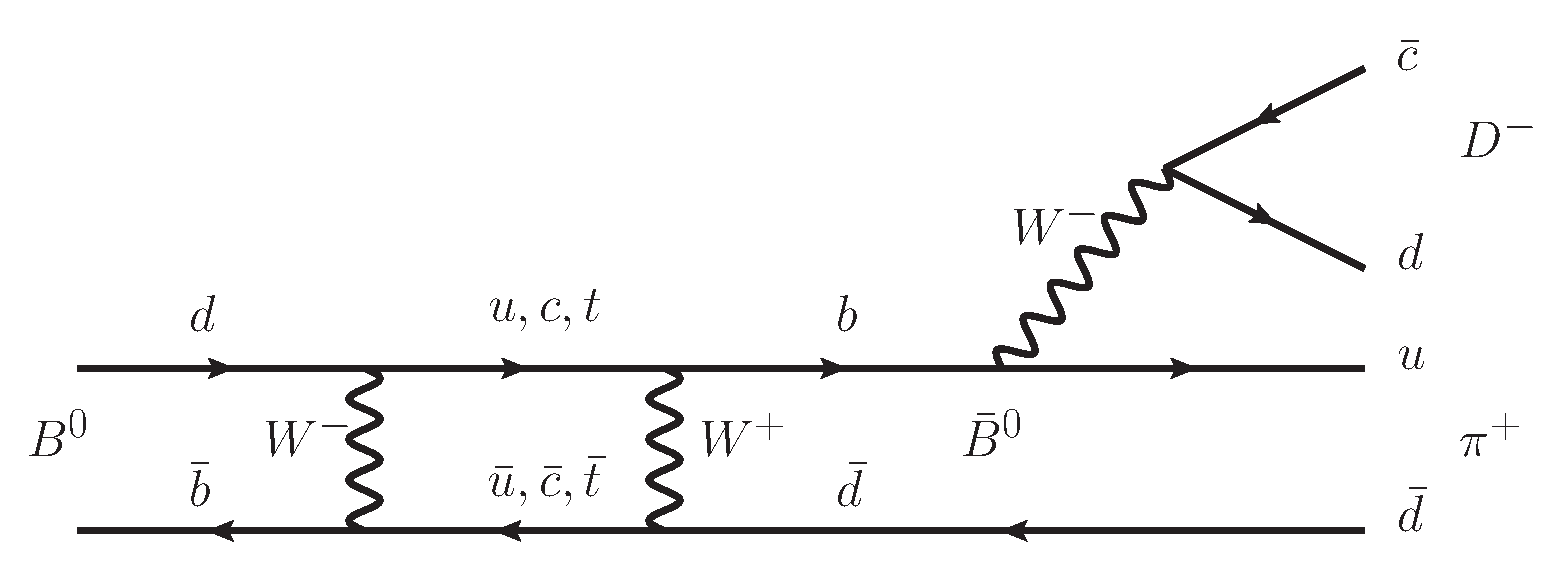
\includegraphics[width=0.8\linewidth]{01Introduction/figs/Mixed.eps}
                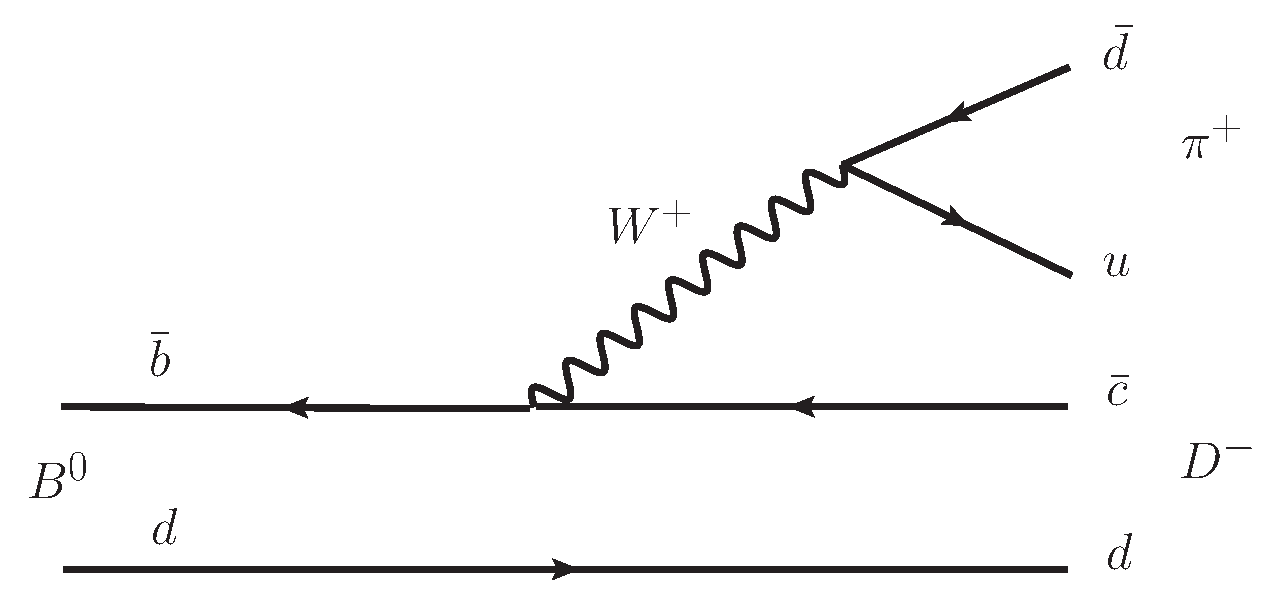
\includegraphics[width=0.7\linewidth]{01Introduction/figs/Unmixed.eps}
                %\vspace*{-1.0cm}                                                                                                           
        \end{center}
        \vspace{-2mm}
        \caption{Feynman diagrams contributing to $\Bz\to \Dm\pip$, with (top) and without (bottom) mixing.}
        \label{fig:Feynman}
        \afterpage{\global\setlength{\textfloatsep}{\oldtextfloatsep}}
\end{figure}
In this thesis, a decay-time dependent analysis of the decay $\Bz\to
\Dmp\pipm$ is presented, where the $\Dpm$ meson is reconstructed as $\Dpm\to\Kmp\pipm\pipm$. The 
pion produced together with the $\Dpm$ meson will be named \emph{bachelor} or \emph{companion} hereafter.
The objective of this study is to perform a
measurement of \CP~asymmetries, in order to constrain the CKM angle
$\gamma$~\cite{PRL-10-1963-531,PTP-49-1973-652}. The $\gamma$ angle is particularly important to test 
the CKM picture of the \CP~violation. In fact, $\gamma$ is the least-known parameter of the UT, whereas 
the theoretical predictions for its value are very clean and free from hadronic uncertainties~\cite{Fleischer:2003yb,Aleksan:1991nh,Dunietz:1987bvsss}. 
So, improving the experimental precision on $\gamma$ is a milestone of the current Flavour Physics programme.
\CP~violation appears in the interference between the Cabibbo favoured $b\to c$
amplitude without mixing, $A(\Bz\to \Dm\pip)$, and the Cabibbo suppressed $b\to u$
amplitude with mixing, $A(\Bz\to\Bzb\to\Dm\pip)$. Two of the corresponding
Feynman diagrams for these amplitudes are depicted in Fig.~\ref{fig:Feynman}.

The measurement is performed by analysing the four time-dependent decay
rates \\
$\frac{d\Gamma(\Bz\to\Dm\pip)}{dt}$, $\frac{d\Gamma(\Bz\to\Dp\pim)}{dt}$, $\frac{d\Gamma(\Bzb\to\Dm\pip)}{dt}$ and $\frac{d\Gamma(\Bzb\to \Dp\pim)}{dt}$. 
Identifying the final state as $f=\Dm\pip$ or $\bar f=\Dp\pim$, and assuming $CPT$ symmetry, no \CP~violation in mixing ($|q/p|=1$) and decay
($|A_f|^2=|\bar A_{\bar f}|^2$, $|A_{\bar f}|^2=|\bar A_f|^2$), and $\Delta\Gamma=0$, the time-dependent decay rates for $B$ mesons initially
produced as $\Bz$ or $\Bzb$ can be written as
\begin{align}
	\frac{d\Gamma(\Bz\to f)}{dt}(t) &= \frac{1}{4\tau} e^{-t/\tau} \left[ 1 + C_{f} \cos\left(\Delta m t\right) - S_{f} \sin\left(\Delta m t\right) \right], \label{eq:decay-rate-Bf}\\
	\frac{d\Gamma(\Bzb\to f)}{dt}(t) &= \frac{1}{4\tau} e^{-t/\tau} \left[ 1 - C_{f} \cos\left(\Delta m t\right) + S_{f} \sin\left(\Delta m t\right) \right],\\
	\frac{d\Gamma(\Bz\to \bar f)}{dt}(t) &= \frac{1}{4\tau} e^{-t/\tau} \left[ 1 + C_{\bar f} \cos\left(\Delta m t\right) - S_{\bar f} \sin\left(\Delta m t\right) \right],\\
	\frac{d\Gamma(\Bzb\to \bar f)}{dt}(t) &= \frac{1}{4\tau} e^{-t/\tau} \left[ 1 - C_{\bar f} \cos\left(\Delta m t\right) + S_{\bar f} \sin\left(\Delta m t\right) \right], \label{eq:decay-rate-Bbfb}
\end{align}
where $\Delta m$ and $\tau=1/\Gamma$ are given by Eqs.~\ref{eq:deltaM} and~\ref{eq:deltaGamma}, respectively.
The \CP~coefficients defined in Eqs.~\ref{eq:cp_f} and~\ref{eq:cp_fbar}, can be expressed as
\begin{align}
	S_{f}&=-\frac{2r_{D\pi}\sin[\delta-(\gamma+2\beta)]}{1+r_{D\pi}^{2}}, & S_{\bar f}&=\frac{2r_{D\pi}\sin[\delta+(\gamma+2\beta)]}{1+r_{D\pi}^{2}}, \\
	C_{f}&=-C_{\bar f}=C=\frac{1-r_{D\pi}^{2}}{1+r_{D\pi}^{2}},
\end{align}
where $\beta$ (Eq.~\ref{eq:alpha_beta}) is related to the $\Bz$ mixing
phase, 
\begin{equation}
  r_{D\pi} = \frac{|\bar A_f|}{|A_f|} = \frac{|A_{\bar f}|}{|\bar A_{\bar f}|}
\end{equation}
is the magnitude of
the ratio between the doubly Cabibbo suppressed and favoured amplitudes, and
$\delta$ is the strong phase difference between these amplitudes.

A measurement of $\gamma$ can be obtained by measuring the \CP~coefficients and
taking external measurements of $\beta$ and $r_{D\pi}$ as input. The angle $\beta$ is
known with very high precision, both theoretically and
experimentally~\cite{LHCb-PAPER-2015-005}. An estimation of $r_{D\pi}$ was performed by the
BaBar and Belle collaborations~\cite{Aubert:2008zi,Das:2010be}, by measuring the
branching fraction of $\Bz\to D_{s}^{(*)+} \pim$ decays and assuming SU(3)
symmetry, yielding an average of about $1.7\%$ with a relative error around
15\%, mainly due to SU(3) symmetry breaking. Because of the very small value of $r_{D\pi}$, 
this analysis is not sensitive to $C_{f}$ and $C_{\bar f}$; for this reason, 
these coefficients are simply fixed to $+1$ and $-1$, respectively.

The small value for the $r_{D\pi}$ parameter, which reduces the sensitivity on $S_{f/\bar f}$, makes this measurement challenging 
as compared to similar analyses like $\Bs\to\Dsmp\Kpm$. 
However, the $\Bs$ production rate is significantly smaller 
than the $\Bz$ production fraction ($f_s/f_d=0.259\pm0.015$~\cite{LHCb:2013lka}). 
Moreover, the $\Bs\to\Dsmp\Kpm$ branching ratio, $(2.27\pm0.19)\times 10^{-4}$~\cite{Louvot:2008sc}, is much smaller than 
the $\Bz\to\Dm\pip$ branching ratio, $(2.52\pm0.13)\times 10^{-3}$~\cite{PDG2017}.  
So, the resulting, larger number of $\Bz\to\Dmp\pipm$ candidates compensates for this reduced sensitivity.

Measurements of $\sin(2\beta+\gamma)$ in $\Bz\to D^{(*)\mp}\pipm$ were performed previously
by the BaBar and Belle collaborations~\cite{Aubert:2006tw,Aubert:2005yf,Bahinipati:2011yq,PhysRevD.73.092003}.
I'm one of the authors of a measurement of $2\beta_s - \gamma$ in $\Bs\to\Dsmp\Kpm$ decays with $3\invfb$ of data~\cite{LHCb-PAPER-2017-047}.

The measurement presented in this thesis is performed in terms of a flavour-tagged, decay-time dependent
analysis of the Run 1 dataset (Sec.~\ref{sec:lhcdata}). The dataset includes two sub-samples recorded with opposite
directions of the magnetic field (``up'' and ``down'') in the spectrometer dipole.
The selection of the decays, which is explained in detail in Sec.~\ref{sec:sample_and_selection}, includes
the use of vetoes to reduce the number of components that must be modelled in the sample, and
a boosted decision tree (BDT) to reduce the amount of \emph{combinatorial} background. The expected sample
composition after the selection is discussed in Sec.~\ref{sec:MC} based on
studies with simulated samples. A fit to the invariant mass distribution of the
resulting dataset is performed to extract \emph{sWeights}~\cite{Pivk:2004ty} for the signal component. The
fit is described in detail in Sec.~\ref{sec:massfit}. The training and
calibration of the flavour-tagging algorithms, which infer the initial flavour
of the reconstructed $\Bz$ candidates, is summarised in
Sec.~\ref{sec:tagging}. Finally, the estimation of the \CP~coefficients is
the result of an unbinned, \emph{sWeighted} likelihood fit to the distributions of the
decay time and the flavour tagging observables. 
